% **************************************************
% Information and Commands for Reuse
% **************************************************
\newcommand{\thesisTitle}{Evaluierung und Implementierung von Server Roundtrip Verfahren unter Gewährleistung der Typsicherheit in einer bestehenden Webapplikation}
\newcommand{\thesisSubtitle}{Bachelor-Thesis im Fachbereich Informatik}
\newcommand{\thesisDate}{26. August 2020}
%\newcommand{\thesisVersion}{\input{GIT_REV}}

\newcommand{\thesisAuthor}{Yannick Schröder}
\newcommand{\thesisAuthorStudentNumber}{Informatik 102751}
\newcommand{\thesisAuthorEmail}{inf102751@fh-wedel.de}

\newcommand{\thesisFirstReviewer}{Dr. Michael Predeschly}
\newcommand{\thesisFirstReviewerEmail}{\protect{mpr@fh-wedel.de}}

\newcommand{\thesisSecondReviewer}{M.~Sc. Marcus Riemer}
\newcommand{\thesisSecondReviewerEmail}{\protect{mri@fh-wedel.de}}

\newcommand{\thesisUniversity}{\protect{Fachhochschule Wedel}}
\newcommand{\thesisUniversityCity}{Wedel}
\newcommand{\thesisUniversityStreetAddress}{Feldstra{\ss}e 143}
\newcommand{\thesisUniversityPostalCode}{22880}

% **************************************************
% Load and Configure Packages
% **************************************************
\usepackage[utf8]{inputenc}       % defines file's character encoding
\usepackage[ngerman]{babel}       % babel system, adjust the language of the content
\usepackage[                      % clean thesis style
	figuresep=colon,%
	sansserif=false,%
	hangfigurecaption=false,%
	hangsection=false,%
	hangsubsection=false,%
	colorize=full,%
	colortheme=bluemagenta,%
	bibsys=bibtex,%
	bibfile=bib-refs,%
	bibstyle=alphabetic,%
]{sty/cleanthesis}

\hypersetup{                      % setup the hyperref-package options
	pdftitle={\thesisTitle},      %   - title (PDF meta)
	pdfsubject={\thesisSubtitle}, %   - subject (PDF meta)
	pdfauthor={\thesisAuthor},    %   - author (PDF meta)
	plainpages=false,             %   -
	colorlinks=false,             %   - colorize links?
	pdfborder={0 0 0},            %   -
	breaklinks=true,              %   - allow line break inside links
	bookmarksnumbered=true,       %
	bookmarksopen=true            %
}

% Font and Color
\cthesissetcolor{cmyk}{1, .87, .27, .12}{1, .87, .27, .12}
\usepackage{fontspec}

% \setmainfont{Dax Pro}
% \renewcommand{\helv}{\fontspec{Dax Pro}\fontsize{12}{14}\selectfont}
% \renewcommand{\book}{\fontspec{Dax Pro}\fontsize{12}{14}\selectfont}
% \renewcommand{\tgherosfont}{\fontspec{Dax Pro}}
% \renewcommand{\thesischapterfont}{\color{ctcolorblack}\huge\fontspec{Dax Pro}}

% \renewcommand{\ttfamily}{\fontspec{Ubuntu Mono}}

\renewcommand{\cftchapfont}{\normalfont\bfseries}
\renewcommand{\cftchappagefont}{\normalfont\bfseries}
\usepackage{multicol}
\addtokomafont{caption}{\normalfont}
\addtokomafont{captionlabel}{\normalfont}
\urlstyle{rm}
\makeatletter
\def\blx@maxline{77}
\makeatother

% **************************************************
% Additional Utilities
% **************************************************

\newcommand{\fullref}[1]{\ref{#1}~\enquote{\nameref{#1}}}


% \inlinec for inline code
\NewDocumentCommand{\inlinec}{v}{%
\texttt{#1}%
}

% Fix quotes
\usepackage{csquotes}
\MakeOuterQuote{"}

% Code
\usepackage{listings,lstautogobble}

\definecolor{lightgray}{rgb}{.9,.9,.9}
\definecolor{darkgray}{rgb}{.4,.4,.4}
\definecolor{purple}{rgb}{0.65, 0.12, 0.82}
\definecolor{orange}{rgb}{1, 0.722, 0.424}

\lstset{
	numberstyle=\tiny
}


\lstdefinelanguage{SQL}{
	keywords={INSERT, UPDATE, DELETE, SELECT, FROM, WHERE, GROUP BY, SET, INTO, VALUES, LIMIT},
	keywordstyle=\color{blue}\bfseries,
	ndkeywords={strftime},
	ndkeywordstyle=\color{OliveGreen}\bfseries,
	identifierstyle=\color{black},
	sensitive=false,
	comment=[l]{//},
	morecomment=[s]{/*}{*/},
	commentstyle=\color{purple}\ttfamily,
	stringstyle=\color{red}\ttfamily,
	morestring=[b]',
	morestring=[b]"
}

\lstdefinelanguage{HTML}{
	keywords={select, option, h1, template, h2, div, ul, li, table, thead, tr, th, td, tbody, tr, value, innerHtml, class, id},
	keywordstyle=\color{blue}\bfseries,
	ndkeywords={for, in, include, endfor, endif, else, if, ngIf, ngFor, each},
	ndkeywordstyle=\color{OliveGreen}\bfseries,
	identifierstyle=\color{black},
	sensitive=false,
	comment=[l]{//},
	morecomment=[s]{/*}{*/},
	commentstyle=\color{purple}\ttfamily,
	stringstyle=\color{red}\ttfamily,
	morestring=[b]',
	morestring=[b]"
}

\lstdefinelanguage{JavaScript}{
	keywords={typeof, new, true, false, catch, function, return, null, catch, switch, var, let, const, if, in, while, do, else, case, break},
	keywordstyle=\color{blue}\bfseries,
	ndkeywords={class, export, boolean, number, string, throw, extends, implements, import, this, constructor, public, private},
	ndkeywordstyle=\color{darkgray}\bfseries,
	identifierstyle=\color{black},
	sensitive=false,
	comment=[l]{//},
	morecomment=[s]{/*}{*/},
	commentstyle=\color{purple}\ttfamily,
	stringstyle=\color{red}\ttfamily,
	morestring=[b]',
	morestring=[b]"
}

\lstdefinelanguage{Ruby}{
	keywords={do, def, end, if, else, return},
	keywordstyle=\color{blue}\bfseries,
	ndkeywords={each, map, zip},
	ndkeywordstyle=\color{darkgray}\bfseries,
	identifierstyle=\color{black},
	sensitive=false,
	comment=[l]{\#},
	morecomment=[s]{/*}{*/},
	commentstyle=\color{purple}\ttfamily,
	stringstyle=\color{red}\ttfamily,
	morestring=[b]',
	morestring=[b]"
}

\lstset{
	backgroundcolor=\color{white},
	extendedchars=true,
	basicstyle=\scriptsize\ttfamily,
	showstringspaces=false,
	showspaces=false,
	numbers=left,
	stepnumber=1,
	numberstyle=\tiny\ttfamily,
	numbersep=9pt,
	tabsize=4,
	breaklines=true,
	showtabs=false,
	captionpos=b,
	autogobble=true,
	frame=single
}



\usepackage[simplified]{sty/pgf-umlcd}
\usepackage{float}

% https://tex.stackexchange.com/a/42620
\usepackage{amssymb}
\usepackage{pifont}
\newcommand{\cmark}{\ding{51}}
\newcommand{\xmark}{\ding{55}}

\usepackage{nameref}
\usepackage[multidot]{grffile}
\usepackage{xparse}

% **************************************************
% Document CONTENT
% **************************************************
\begin{document}

% --------------------------
% rename document parts
% --------------------------
\renewcaptionname{ngerman}{\figurename}{Abb.}
\renewcaptionname{ngerman}{\tablename}{Tab.}

% --------------------------
% Front matter
% --------------------------
\pagenumbering{roman}             % roman page numbing (invisible for empty page style)
\pagestyle{empty}                 % no header or footers
%************************************************
% Titlepages
%************************************************
% ------------------------------------  --> cover title page
\begin{titlepage}
	\pdfbookmark[0]{Cover}{Cover}
	\flushright
	\hfill
	\vfill
	{\LARGE\thesisTitle \par}
	\rule[5pt]{\textwidth}{.4pt} \par
	{\Large\thesisAuthor}
	\vfill
	\textit{\large\thesisDate} \\
	Version: \thesisVersion
\end{titlepage}


% ------------------------------------  --> main title page
\begin{titlepage}
	\pdfbookmark[0]{Titelseite}{Titelseite}
	\tgherosfont
	\centering

	
\includegraphics[width=6cm]{gfx/fhw} \\

	\vfill
	{\LARGE \color{ctcolortitle}\textbf{\thesisTitle} \\[10mm]}
	{\Large \thesisSubtitle} \\

	\vfill
	\begin{minipage}[t]{.27\textwidth}
		\raggedleft
		\textit{Autor}
	\end{minipage}
	\hspace*{15pt}
	\begin{minipage}[t]{.65\textwidth}
		{\Large \thesisAuthor} \\
	  	{\thesisAuthorStudentNumber} \\
	  	{\thesisAuthorEmail} \\
    \end{minipage} \\[5mm]
    \begin{minipage}[t]{.27\textwidth}
		\raggedleft
		\textit{Erstgutachter}
	\end{minipage}
	\hspace*{15pt}
	\begin{minipage}[t]{.65\textwidth}
		{\Large \thesisFirstReviewer} \\
	  	{\thesisFirstReviewerEmail} \\
	\end{minipage} \\[5mm]
	\begin{minipage}[t]{.27\textwidth}
		\raggedleft
		\textit{Zweitgutachter}
	\end{minipage}
	\hspace*{15pt}
	\begin{minipage}[t]{.65\textwidth}
		{\Large \thesisSecondReviewer} \\
	  	{\thesisSecondReviewerEmail} \\
	\end{minipage} \\[10mm]
	\begin{minipage}[t]{.27\textwidth}
		\raggedleft
		\textit{Eingereicht am}
	\end{minipage}
	\hspace*{15pt}
	\begin{minipage}[t]{.65\textwidth}
		\thesisDate
	\end{minipage} \\

\end{titlepage}


% ------------------------------------  --> lower title back for single page layout
\hfill
\vfill
{
	\small
	\textbf{\thesisAuthor} \\
	\textit{\thesisTitle} \\
	\thesisSubtitle, \thesisDate \\
    Gutachter: \thesisFirstReviewer\ und \thesisSecondReviewer

	\textbf{\thesisUniversity} \\
	\thesisUniversityStreetAddress \\
	\thesisUniversityPostalCode\ \thesisUniversityCity
}
        % INCLUDE: all titlepages
\cleardoublepage
%
\pagestyle{plain}                 % display just page numbers
%\begin{titlepage}

\section*{Abstrakt}

Konventionelle Entwicklungsumgebungen sind speziell auf die Bedürfnisse von professionellen Programmierern zugeschnittene Programme. Aufgrund der damit verbundenen Komplexität sind sie aus didaktischer Sicht nicht für die Einführung in die Programmierung geeignet. Diese Thesis beschreibt daher ein Konzept und die prototypische Implementierung einer Lehr-Entwicklungsumgebung names \idename{} für Datenbanken und Webseiten. Um syntaktische Fehler während der Programmierung systematisch auszuschließen, werden die Bestandteile der dafür benötigten Programmier- oder Textauszeichnungssprachen ähnlich wie in der Lehrsoftware "`Scratch"' grafisch durch Blockstrukturen repräsentiert. Diese Blöcke lassen sich über Drag \& Drop-Operationen miteinander kombinieren, die syntaktischen Strukturen von \texttt{SQL} und \texttt{HTML} sind für Lernende dabei stets sichtbar, müssen aber noch nicht verinnerlicht werden. So lassen sich auch ohne die manuelle Eingabe von Codezeilen eigene Webseiten programmieren, welche dann im Freundes- und Bekanntenkreis weitergegeben werden können. Für den Unterrichtseinsatz ist der aktuelle Entwicklungsstand von \idename{} allerdings noch nicht geeignet, er dient vornehmlich der Erprobung und Demonstration der erdachten Konzepte.

\section*{Abstract}

Conventional development environments are programs that are tailored to suit the needs of professionals. Due to their complexity they do not lend themselves well to introduce people to programming. This thesis therefore describes the concept and the prototypical implementation of an educational software named \idename{} (a loose translation of the english term ``Page Tool'') for database- and web-development. To eliminate the possibility of syntactical errors while programming, the elements of the programming- or markup-languages are represented by graphical blocks, similar to the approach taken by the software ``Scratch''. These blocks can be combined by using drag \& drop operations. The syntactical structures of \texttt{SQL} and \texttt{HTML} are not hidden from the user, but it is not mandatory to internalize them. This approach allows pupils to program and share their own websites, without the need to type lines of code. The current implementation of this software is not yet ready to be used in a classroom. It's main purpose is to demonstrate and field test the described concepts.

\end{titlepage}

%%% Local Variables:
%%% mode: latex
%%% TeX-master: "thesis"
%%% End:
          % INCLUDE: the abstracts (english and german)
\cleardoublepage
%
\pdfbookmark[0]{Inhaltsverzeichnis}{Inhaltsverzeichnis}
\setcounter{tocdepth}{2}          % define depth of toc
\tableofcontents                  % display table of contents
\cleardoublepage

% --------------------------
% Body matter
% --------------------------
\pagenumbering{arabic}            % arabic page numbering
\setcounter{page}{1}              % set page counter
\pagestyle{maincontentstyle}      % fancy header and footer

%************************************************
% Einleitung
%************************************************
\chapter{Einleitung}
\label{sec:intro}

Mehr als 90 Prozent der Befragten im Alter von 14 bis 29 Jahren sind der Meinung, dass Programmierfähigkeiten vielfältige Möglichkeiten eröffnen, die Welt von Morgen mitzugestalten~\cite{statista-1}. Auch in der Politik wird in Zeiten der Digitalisierung die Forderung nach der Vermittlung von Programmierfähigkeiten für alle Schüler\footnote{Aus Gründen der Lesbarkeit werden Personengruppen in einer Form bezeichnet, wobei immer sowohl weibliche als auch männliche Personen gemeint sind.} immer lauter. Die daraus resultierende Aufgabe stellt Lehrer vor große Herausforderungen. Klassische Programmiersprachen wie Java oder Python bringen einen großen Sprachumfang mit, der Anfänger schnell überfordert~\cite{ko2004}. Simple Eingabe-Ausgabe-Programme, wie sie in diesen Sprachen oft zur Einführung entwickelt werden, da die Einarbeitung in komplizierte Grafik-Bibliotheken selbst für erfahrene Entwickler in der Regel eine recht steile Lernkurve mit sich bringt, frustrieren die Schüler direkt am Anfang~\cite[63]{resnick2009}.

Aus diesem Grund wurden Anwendungen geschaffen, die Anfänger beim Einstieg in die Programmierung unterstützen sollen. Viele dieser Anwendungen, wie z.~B. die Turtle Grafiken (siehe \ref{sec:related:turtle}), erwarten aber weiterhin die Eingabe von getipptem Programmcode, der sich an bestimmte Regeln -- die sogenannte Syntax -- halten muss, damit er ausgeführt werden kann. Auch das Wissen, an welchen Stellen, welcher Befehl einzusetzen ist, muss zunächst gelernt werden. Diese Einstiegshürden führen dazu, dass Schüler schnell das Interesse am Programmieren verlieren~\cite{ko2004}.

Andere Anwendungen versuchen, dies zu vermeiden, indem sie mit syntaxfreier Programmierung wie z.~B. Lightbot (siehe \ref{sec:related:lightbot}) den Code hinter bunten Blöcken und Grafiken verstecken. Dieser Ansatz kann Syntaxfehlern entgegenwirken und die Schüler mit schnell sichtbaren Ergebnissen motivieren. Durch eine Abstraktion der Programmierkonzepte erschweren sie allerdings den späteren Umstieg auf eine echte Programmiersprache~\cite{gouws2013}.

Marcus Riemer liefert mit seiner Masterarbeit BlattWerkzeug einen Ansatz, die Lücke dazwischen zu schließen. Er entwickelte eine Anwendung, welche es Anfängern ermöglicht, Programme mit der Maus aus Blöcken zusammenzustellen, dabei die Anmutung von Programmcode allerdings nicht verschleiert und so die Vorteile beider Vorgehensweisen unter einem Dach zusammenbringt. BlattWerkzeug bietet dank der syntaxfreien Programmierung einen unterstützenden Einstieg, führt dem Neuling aber von Anfang an den Code vor Augen.

Bisher beschränkte sich BlattWerkzeug jedoch auf die Programmierung von Datenbankabfragen und die Zusammenstellung einfacher Bedienoberflächen. Diese Bachelorarbeit beschäftigt sich nun mit der Konzeption und Implementierung einer Erweiterung der Plattform um eine Minisprache -- einer Programmiersprache mit reduziertem Sprachumfang -- welche Neulinge an die Grundkonzepte des Programmierens heranführen soll. In einer Mikrowelt, einer Art virtuellem Spielfeld, sind mit den selbst gebauten Programmen kleine Puzzle Rätsel zu lösen, wodurch die Ausführung der Programmbefehle sichtbar gemacht wird.

Das Kapitel \ref{sec:basics} führt in die für diese Arbeit benötigten Grundlagen ein. Im Kapitel \ref{sec:related} werden anschließend vergleichbare Arbeiten vorgestellt, welche dieser Arbeit als Inspiration gedient haben. Die vorgestellten Arbeiten sind chronologisch ihrer Entstehung nach geordnet und zeichnen so auch den Werdegang dieses Genres auf.

Kapitel \ref{sec:requirements} stellt Anforderungen an die entwickelte Software auf, welche sich aus den Anforderungen an die im Grundlagenkapitel erläuterten Minisprachen und Mikrowelten aus der Literatur, des bestehenden BlattWerkzeug-Projektes und der Aufgabenstellung bei der Vergabe dieses Themas ergeben.

Die Umsetzung dieser Anforderungen und die damit verbundenen Entscheidungen zu Vorgehensweisen, Softwarearchitektur und eingesetzten technischen Methoden werden in Kapitel \ref{sec:implementation} dargestellt. Im Kapitel \ref{sec:conclusion} werden die Anforderungen den erreichten Zielen gegenübergestellt und ein Ausblick gegeben, durch welche Erweiterungen das Ergebnis dieser Arbeit in Zukunft noch weiter verbessert werden könnte.

% \begin{figure}[H]
%   \begin{subfigure}[b]{0.30\textwidth}
%     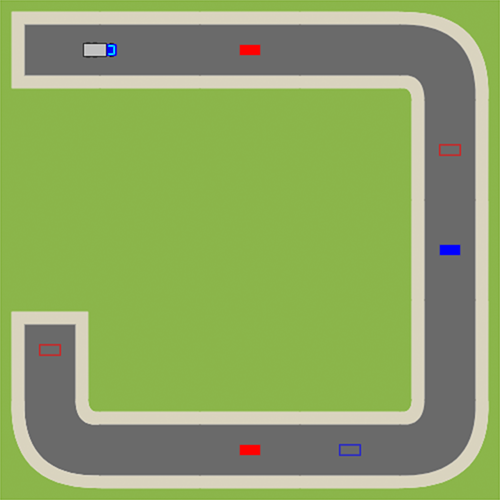
\includegraphics[width=\textwidth]{gfx/exercises-world-d.png}
%     \caption{Beispiel einer Mikrowelt}
%   \end{subfigure}\hfill
%   \begin{subfigure}[b]{0.30\textwidth}
%     \includegraphics[width=\textwidth]{gfx/exercises-program-5.png}
%     \caption{Beispiel eines Programms, welches die Welt löst}
%   \end{subfigure}\hfill
%   \caption{Beispiel Mikrowelt und Minisprache}
% \end{figure}


\appendix{}

%************************************************
% Literaturverzeichnis
%************************************************
\chapter{Literaturverzeichnis}
{%
\setstretch{1.1}
\renewcommand{\bibfont}{\normalfont\small}
\setlength{\biblabelsep}{0pt}
\setlength{\bibitemsep}{0.5\baselineskip plus 0.5\baselineskip}
% \printbibliography
\printbibliography[heading=none,title=Literaturverzeichnis,nottype=online]
\printbibliography[heading=subbibliography,title={Quellen im Internet},type=online,prefixnumbers={@}]
}
\cleardoublepage

%%************************************************
% Beispielaufgaben
%************************************************
\chapter{Beispielaufgaben}
\label{sec:exercises}

Die Anwendungsmöglichkeiten der Software sollen im Folgenden durch eine Reihe von Beispielaufgaben verdeutlicht werden. Die Aufgaben sind nicht geeignet von Schülern alleine gelöst zu werden. Es bedarf einer ausführlichen Einführung und die in den Aufgaben benötigten Konzepte müssen vorab durch eine Lehrkraft erklärt werden. Zusätzlich zum Bildschirmfoto der Musterlösung steht ein Video zur Verfügung, indem die Musterlösung gebaut und ausgeführt wird. Die Musterlösungen stellen i.~d.~R. nur eine von vielen Wegen dar die Aufgabe zu lösen.

\section{Aufgabe 1}
\label{sec:exercises:1}

Dein Lastwagen ist bereits beladen. Fahre zum Ablageplatz und lade den Container ab. Löse die Aufgabe, indem Du zwei Befehle hintereinander ausführst.

\begin{description}[noitemsep]
  \item[Welt wählen:] Welt A
  \item[Du brauchst:] Befehle
  \item[Video:] \url{https://vimeo.com/315544834} (Passwort: trucklino)
\end{description}

\begin{figure}[H]
  \begin{subfigure}[b]{0.40\textwidth}
    \includegraphics[width=\textwidth]{gfx/exercises-world-a.png}
    \caption{Welt A}
  \end{subfigure}\hfill
  \begin{subfigure}[b]{0.40\textwidth}
    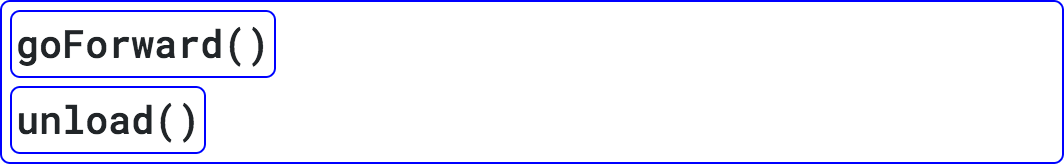
\includegraphics[width=\textwidth]{gfx/exercises-program-1.png}
    \caption{Musterlösung zu Aufgabe 1}
  \end{subfigure}\hfill
  \caption{Welt und Musterlösung zu Aufgabe 1}
\end{figure}

\pagebreak

\section{Aufgabe 2}
\label{sec:exercises:2}

Dieses Mal musst Du die Fracht erst aufladen. Dein Weg enthält außerdem eine Kurve. Reihe mehrere Befehle aneinander, um die Aufgabe zu lösen.

\begin{description}[noitemsep]
  \item[Welt wählen:] Welt B
  \item[Du brauchst:] Befehle
  \item[Video:] \url{https://vimeo.com/315545287} (Passwort: trucklino)
\end{description}

\begin{figure}[H]
  \begin{subfigure}[b]{0.40\textwidth}
    \includegraphics[width=\textwidth]{gfx/exercises-world-b.png}
    \caption{Welt B}
  \end{subfigure}\hfill
  \begin{subfigure}[b]{0.40\textwidth}
    \includegraphics[width=\textwidth]{gfx/exercises-program-2.png}
    \caption{Musterlösung zu Aufgabe 2}
  \end{subfigure}\hfill
  \caption{Welt und Musterlösung zu Aufgabe 2}
\end{figure}

\pagebreak

\section{Aufgabe 3}
\label{sec:exercises:3}

Erkennst Du das Muster? Wenn Du Deine Befehle in einer Prozedur verpackst, bleibt Dein Programm kurz und übersichtlich.

\begin{description}[noitemsep]
  \item[Welt wählen:] Welt C
  \item[Du brauchst:] Befehle, eigene Prozeduren
  \item[Video:] \url{https://vimeo.com/315545769} (Passwort: trucklino)
\end{description}

\begin{figure}[H]
  \begin{subfigure}[b]{0.40\textwidth}
    \includegraphics[width=\textwidth]{gfx/exercises-world-c.png}
    \caption{Welt C}
  \end{subfigure}\hfill
  \begin{subfigure}[b]{0.40\textwidth}
    \includegraphics[width=\textwidth]{gfx/exercises-program-3.png}
    \caption{Musterlösung zu Aufgabe 3}
  \end{subfigure}\hfill
  \caption{Welt und Musterlösung zu Aufgabe 3}
\end{figure}

\pagebreak

\section{Aufgabe 4}
\label{sec:exercises:4}

Deine Prozedur kannst Du auch in einer Zählerschleife mehrmals hintereinander ausführen.

\begin{description}[noitemsep]
  \item[Welt wählen:] Welt C
  \item[Du brauchst:] Befehle, eigene Prozeduren, Zählerschleife
  \item[Video:] \url{https://vimeo.com/315545858} (Passwort: trucklino)
\end{description}

\begin{figure}[H]
  \begin{subfigure}[b]{0.40\textwidth}
    \includegraphics[width=\textwidth]{gfx/exercises-world-c.png}
    \caption{Welt C}
  \end{subfigure}\hfill
  \begin{subfigure}[b]{0.40\textwidth}
    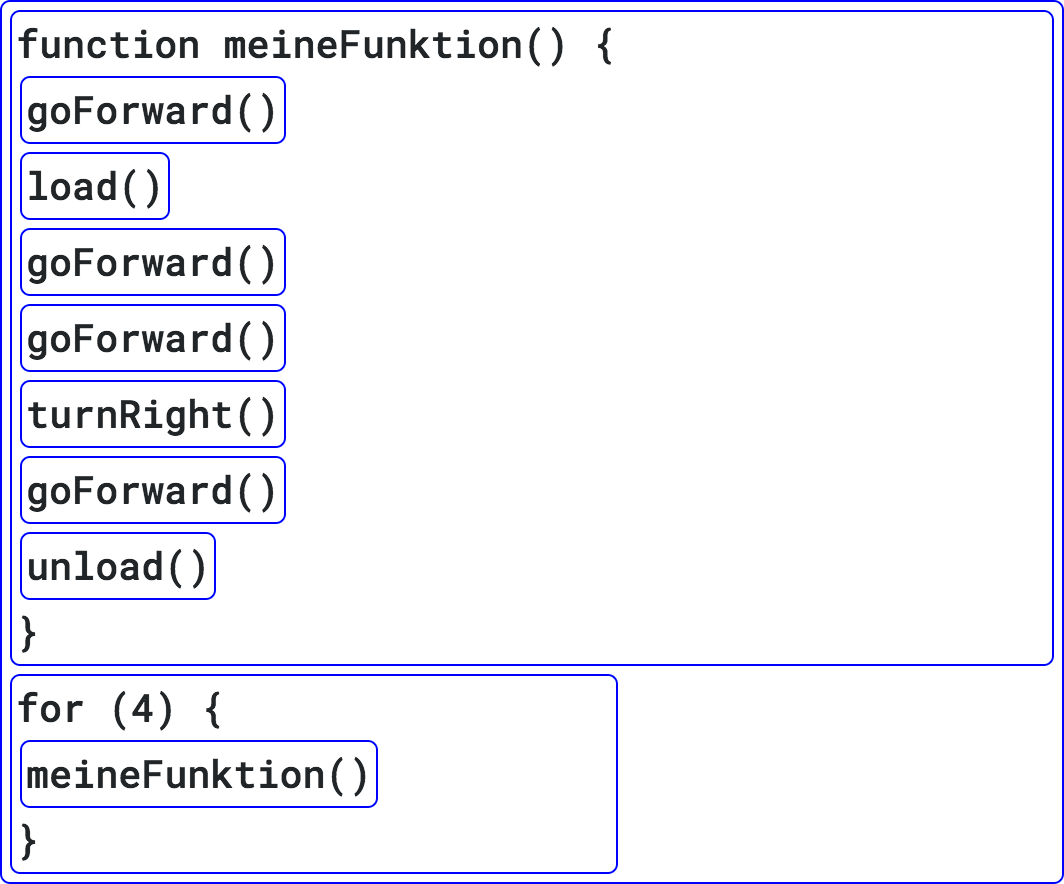
\includegraphics[width=\textwidth]{gfx/exercises-program-4.png}
    \caption{Musterlösung zu Aufgabe 4}
  \end{subfigure}\hfill
  \caption{Welt und Musterlösung zu Aufgabe 4}
\end{figure}

\pagebreak

\section{Aufgabe 5}
\label{sec:exercises:5}

Was passiert, wenn Du nicht weißt, wie oft Du Deine Prozedur ausführen musst? Benutze Sensoren und eine abweisende Schleife, um Deine Prozedur mehrmals auszuführen. Teste Dein Programm mit Welt B, C und D.

\begin{description}[noitemsep]
  \item[Welt wählen:] Welt B, Welt C, Welt D
  \item[Du brauchst:] Befehle, eigene Prozeduren, Sensoren, abweisende Schleife
  \item[Video:] \url{https://vimeo.com/315545914} (Passwort: trucklino)
\end{description}

\begin{figure}[H]
  \begin{subfigure}[b]{0.40\textwidth}
    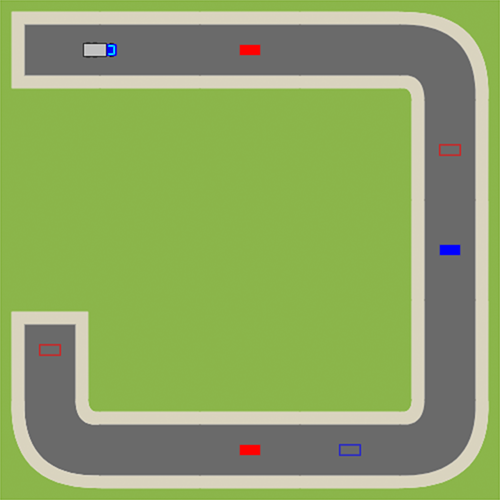
\includegraphics[width=\textwidth]{gfx/exercises-world-d.png}
    \caption{Welt D}
  \end{subfigure}\hfill
  \begin{subfigure}[b]{0.40\textwidth}
    \includegraphics[width=\textwidth]{gfx/exercises-program-5.png}
    \caption{Musterlösung zu Aufgabe 5}
  \end{subfigure}\hfill
  \caption{Welt und Musterlösung zu Aufgabe 5}
\end{figure}

\pagebreak

\section{Aufgabe 6}
\label{sec:exercises:6}

Statt einer abweisenden Schleife kannst Du auch Rekursion benutzen. Benutze eine Verzweigung, um Deine Prozedur im richtigen Moment zu verlassen.

\begin{description}[noitemsep]
  \item[Welt wählen:] Welt B, Welt C, Welt D
  \item[Du brauchst:] Befehle, eigene Prozeduren, Sensoren, Verzweigungen
  \item[Video:] \url{https://vimeo.com/315545989} (Passwort: trucklino)
\end{description}

\begin{figure}[H]
  \begin{subfigure}[b]{0.40\textwidth}
    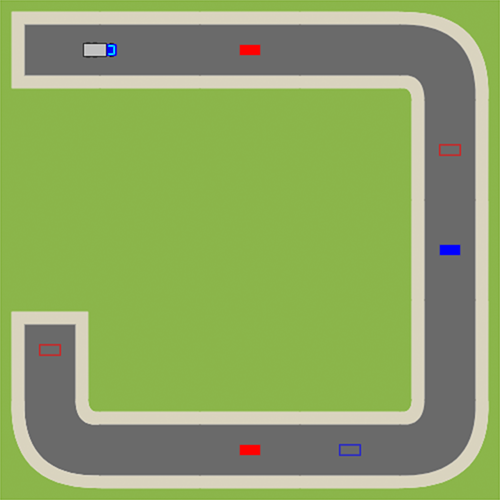
\includegraphics[width=\textwidth]{gfx/exercises-world-d.png}
    \caption{Welt D}
  \end{subfigure}\hfill
  \begin{subfigure}[b]{0.40\textwidth}
    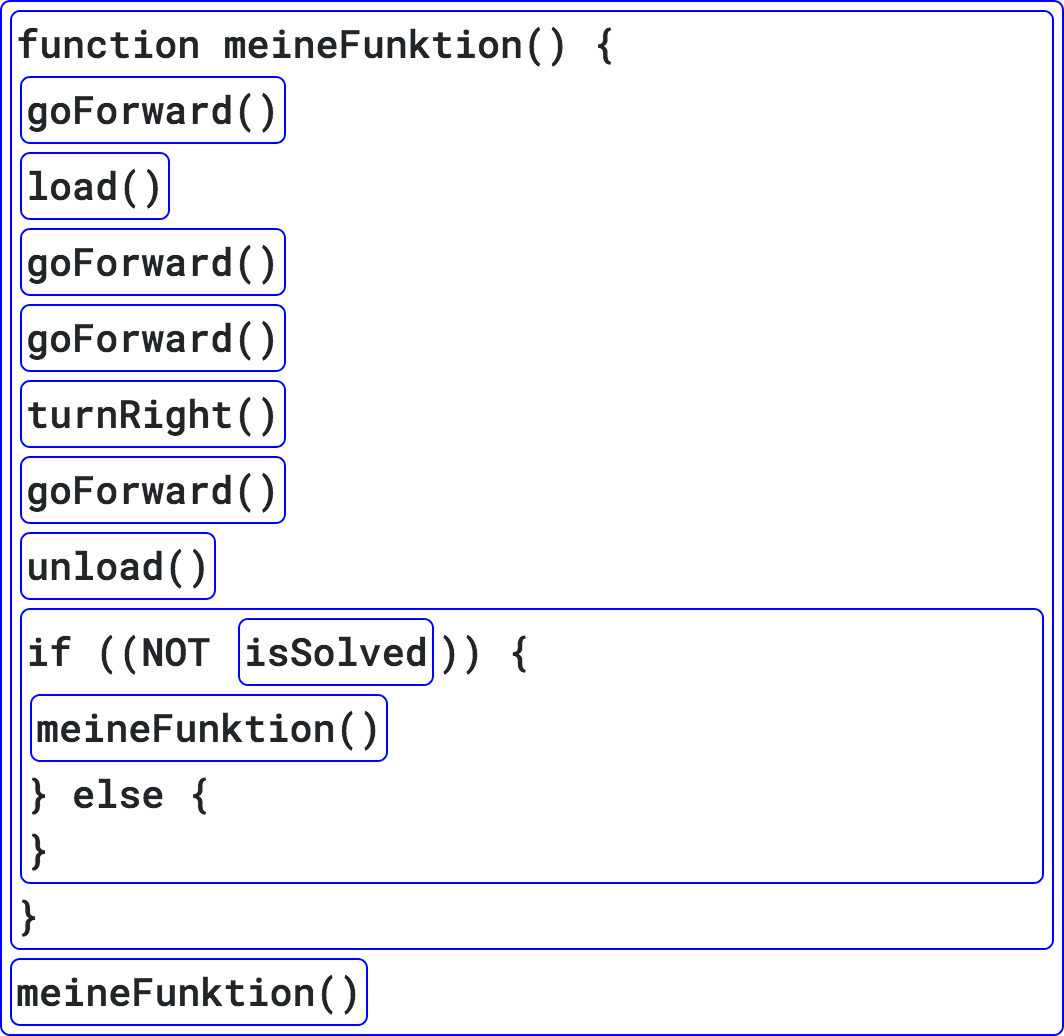
\includegraphics[width=\textwidth]{gfx/exercises-program-6.png}
    \caption{Musterlösung zu Aufgabe 6}
  \end{subfigure}\hfill
  \caption{Welt und Musterlösung zu Aufgabe 6}
\end{figure}

\pagebreak

\section{Aufgabe 7}
\label{sec:exercises:7}

Baue eine eigene Prozedur, die nicht nur geradeaus, sondern auch durch Kurven fahren kann. Deine Prozedur kannst Du solange aufrufen, bis Du am Ziel bist. Benutze dafür entweder eine abweisende Schleife oder Rekursion. Wenn Dein Programm mit Welt E funktioniert, probiere auch Welt F aus.

\begin{description}[noitemsep]
  \item[Welt wählen:] Welt E, Welt F
  \item[Du brauchst:] Befehle, eigene Prozeduren, Sensoren, Verzweigungen, abweisende Schleife (optional)
  \item[Video:] \url{https://vimeo.com/315546116} (Passwort: trucklino)
\end{description}

\begin{figure}[H]
  \begin{subfigure}[b]{0.40\textwidth}
    \includegraphics[width=\textwidth]{gfx/exercises-world-e.png}
    \caption{Welt E}
  \end{subfigure}\hfill
  \begin{subfigure}[b]{0.40\textwidth}
    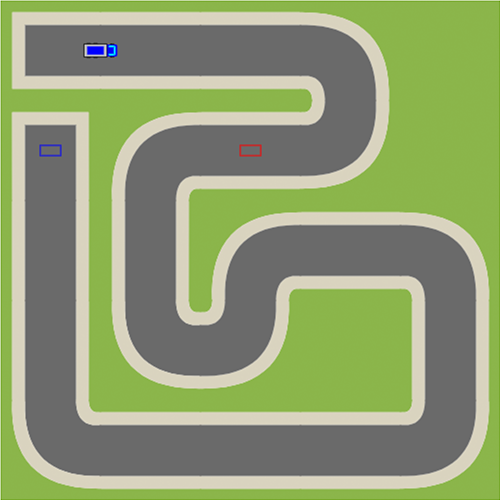
\includegraphics[width=\textwidth]{gfx/exercises-world-f.png}
    \caption{Welt F}
  \end{subfigure}\hfill
  \vspace{0.5cm}
  \begin{subfigure}[b]{0.40\textwidth}
    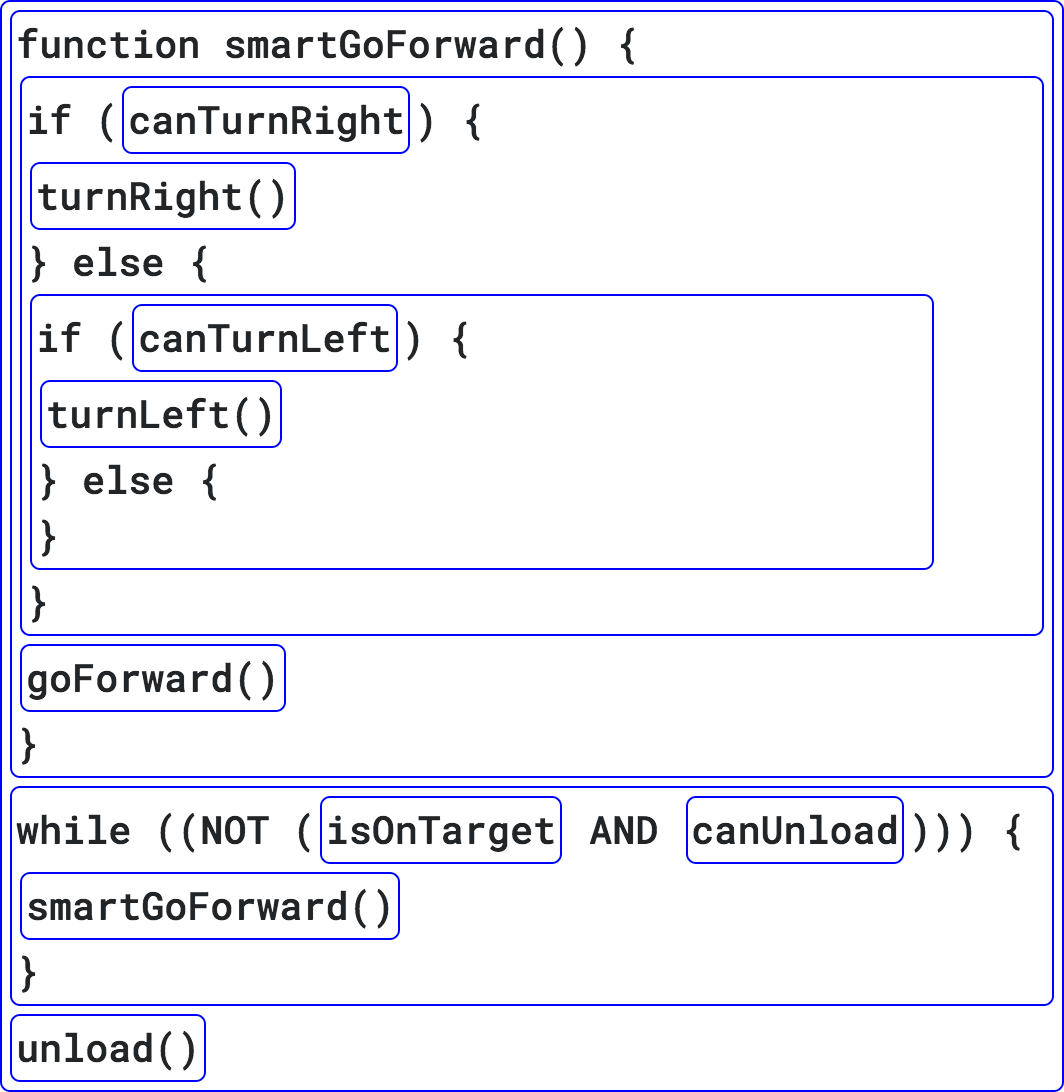
\includegraphics[width=\textwidth]{gfx/exercises-program-7.png}
    \caption{Musterlösung zu Aufgabe 7}
  \end{subfigure}\hfill
  \caption{Welten und Musterlösung zu Aufgabe 7}
\end{figure}

\pagebreak

\section{Aufgabe 8}
\label{sec:exercises:8}

Auf dem Weg sind nun einige Ampeln. Baue Dir eine zusätzliche Prozedur, die wartet, bis es grün wird.

\begin{description}[noitemsep]
  \item[Welt wählen:] Welt G
  \item[Du brauchst:] Befehle, eigene Prozeduren, Sensoren, Verzweigungen, abweisende Schleife (optional)
  \item[Video:] \url{https://vimeo.com/315546210} (Passwort: trucklino)
\end{description}

\begin{figure}[H]
  \begin{subfigure}[b]{0.40\textwidth}
    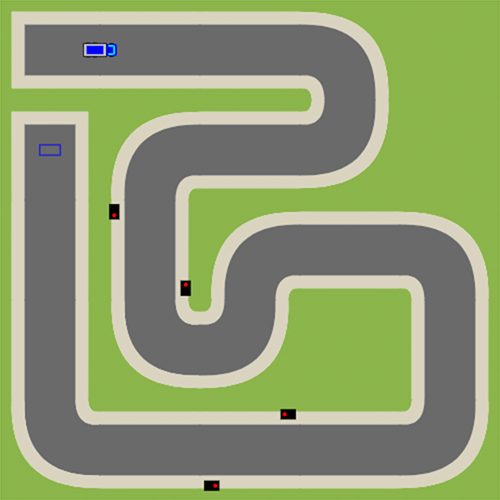
\includegraphics[width=\textwidth]{gfx/exercises-world-g.png}
    \caption{Welt G}
  \end{subfigure}\hfill
  \begin{subfigure}[b]{0.40\textwidth}
    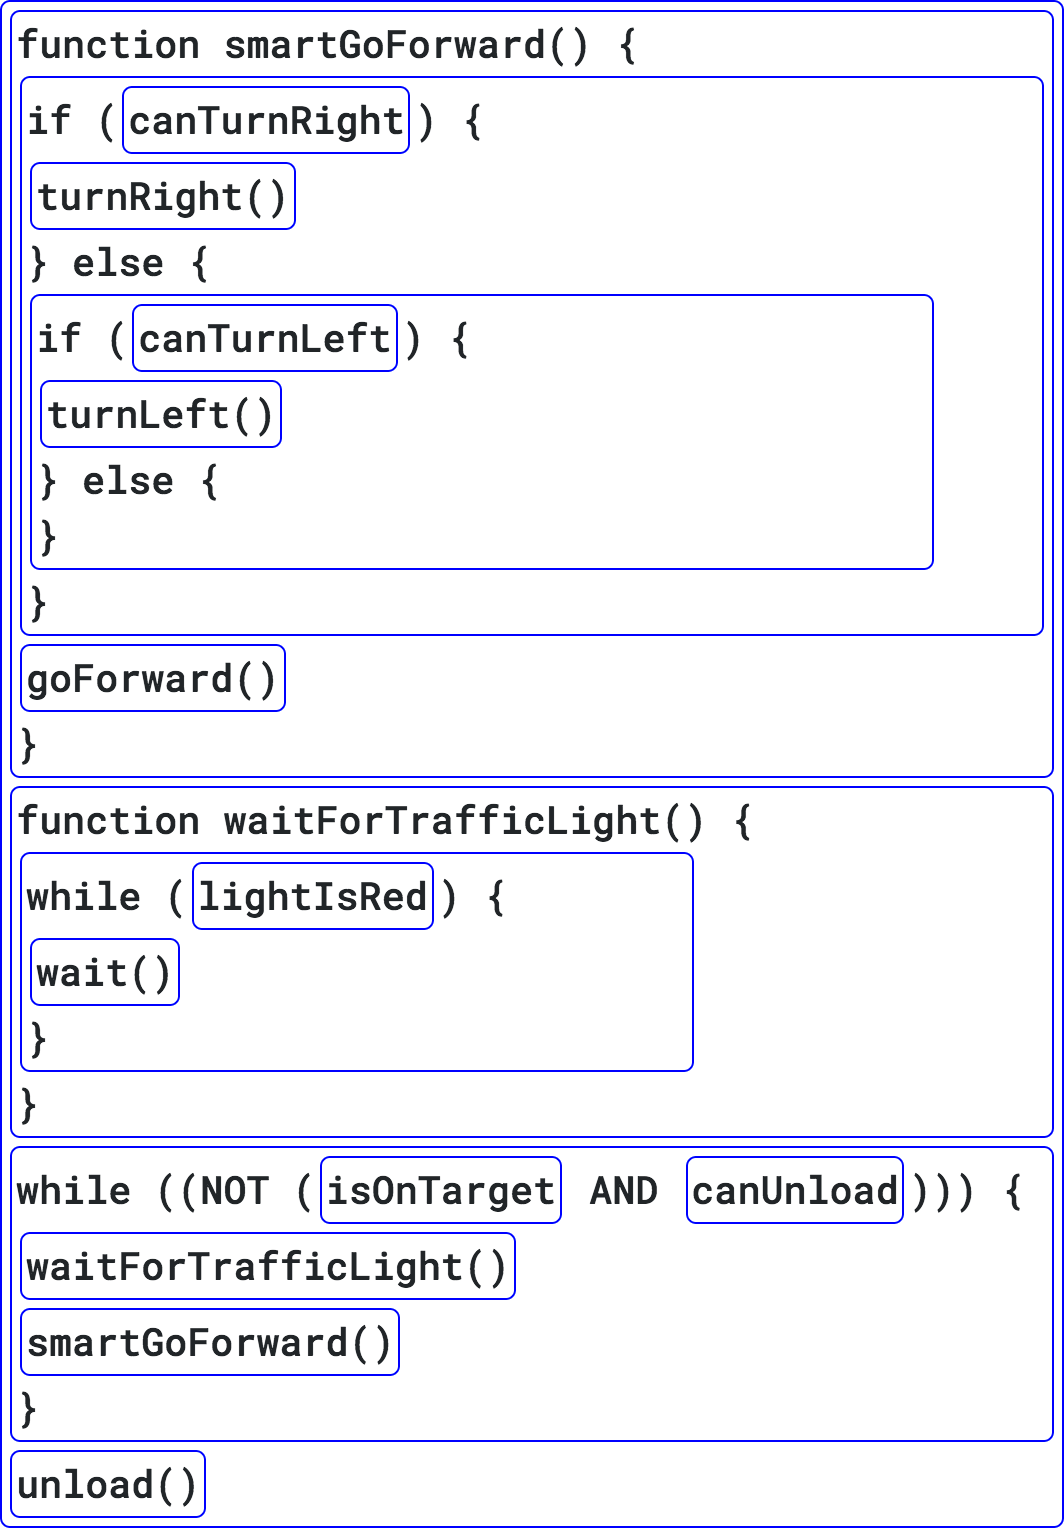
\includegraphics[width=\textwidth]{gfx/exercises-program-8.png}
    \caption{Musterlösung zu Aufgabe 8}
  \end{subfigure}\hfill
  \caption{Welt und Musterlösung zu Aufgabe 8}
\end{figure}

%%************************************************
% CD-ROM
%************************************************
\chapter{CD-ROM}
\label{sec:cd-rom}

Alle auf der beigefügten CD-ROM enthaltenen Daten sind auch im BlattWerkzeug-Git-Repository unter \url{http://blattwerkzeug.de/forward/git-repository} verfügbar.


% \listoffigures
% \cleardoublepage

% \listoftables
% \cleardoublepage

%************************************************
% Declaration
%************************************************
% \pdfbookmark[0]{Eidesstattliche Erklärung}{Eidesstattliche Erklärung}
\chapter{Eidesstattliche Erklärung}
\label{sec:declaration}
\thispagestyle{empty}

Ich erkläre hiermit an Eides statt, dass ich die vorliegende Arbeit selbstständig und ohne Benutzung anderer als der angegebenen Hilfsmittel angefertigt habe; die aus fremden Quellen direkt oder indirekt übernommenen Gedanken sind als solche kenntlich gemacht. Die Arbeit wurde bisher in ähnlicher Form keiner anderen Prüfungskommission vorgelegt und auch nicht veröffentlicht.

\bigskip
\bigskip
\bigskip
\bigskip

\begin{multicols}{2}
    \raggedright
    \thesisUniversityCity, \thesisDate

    \raggedleft
    \thesisAuthor
\end{multicols}

\cleardoublepage
